\documentclass{article}

\usepackage{graphicx}
\usepackage{tikz}
\usepackage{tikzsymbols}
\usetikzlibrary{calc,patterns,shapes.geometric}
\pagestyle{empty}
\usepackage[margin=0pt]{geometry}
\geometry{papersize={14in,12in}}

\def\centerarc[#1](#2)(#3:#4:#5){\draw[#1] ($(#2)+({#5*cos(#3)},{#5*sin(#3)})$) arc (#3:#4:#5);}

\begin{document}
	\begin{figure}
		\centering
		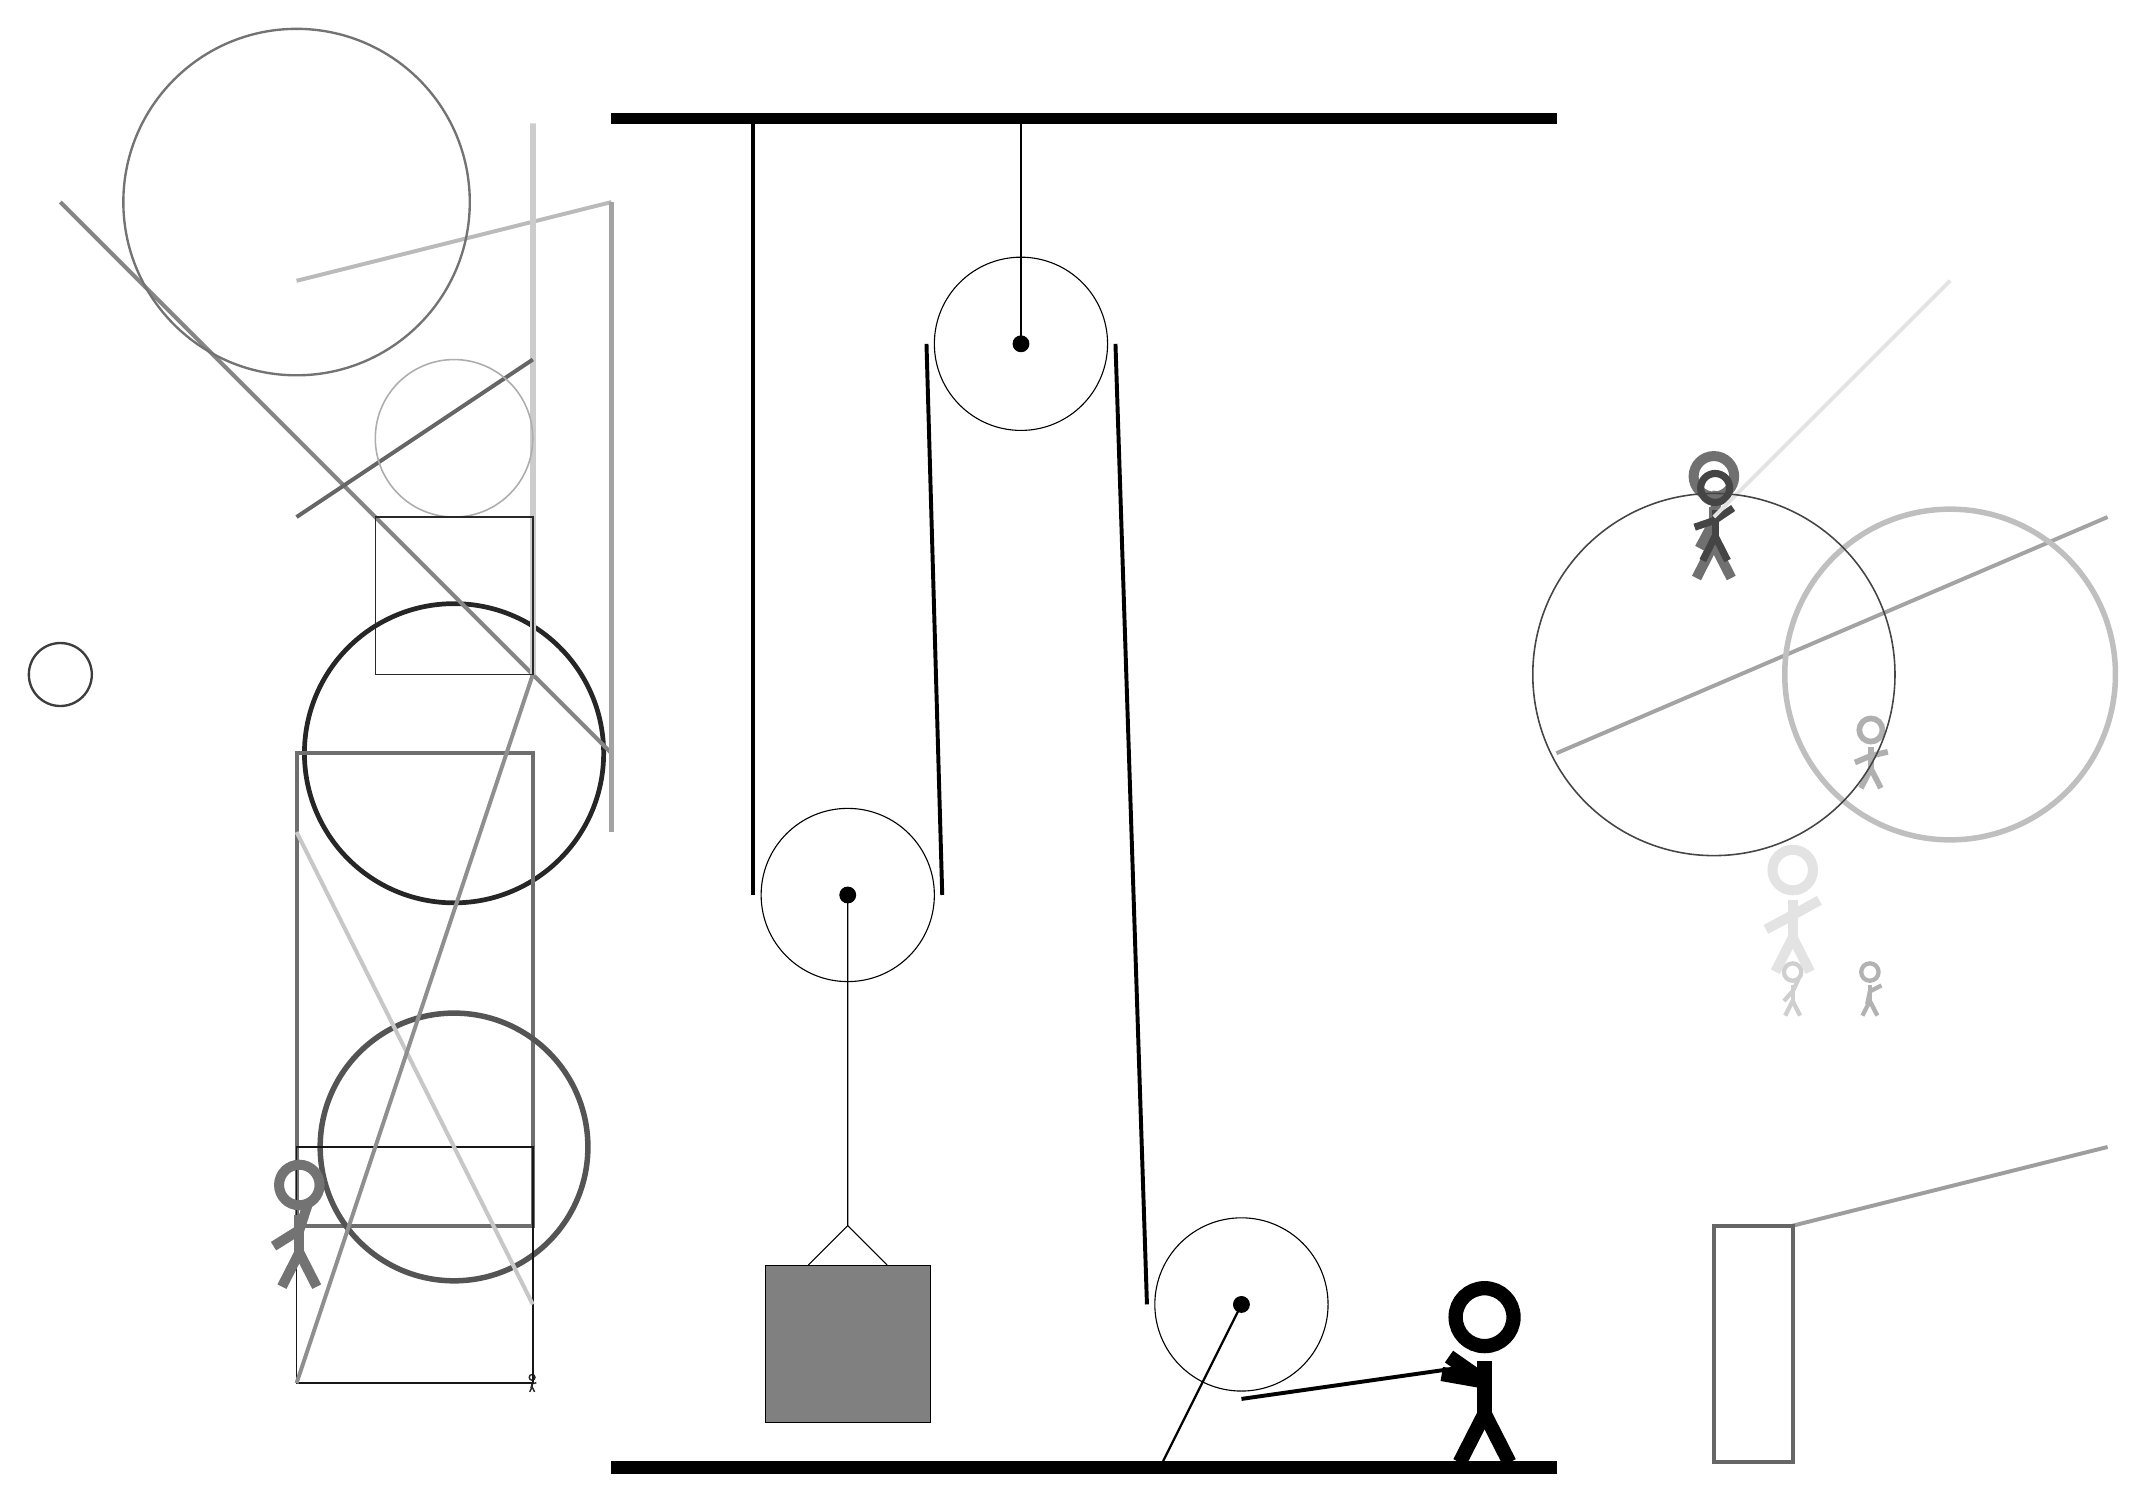
\begin{tikzpicture}
			%%%%% START %%%%%
			
			\draw[fill=black] (-2, 14) rectangle (10, 14.125);
			
			\draw (3.2, 11.2) circle (1.1);
			\draw[fill=black] (3.2, 11.2) circle (0.1);
			\draw[thick] (3.2, 11.2) -- (3.2, 14);
			
			\draw (6, -1) circle (1.1);
			\draw[fill=black] (6, -1) circle (0.1);
			\draw[thick] (6, -1) -- (5, -3);
			
			\draw[line width=0.5mm, color=black!36](10, 6) -- (17, 9);
			
			\node[line width=0.4mm, color=black!84] at (-3, -2) {\Strichmaxerl[1][75][14]};
			\node[line width=0.4mm, color=black!19] at (13, 3) {\Strichmaxerl[3][48][64]};
			\draw [line width=0.6mm, color=black!85](-4, 6) circle (1.9);
			\node[line width=0.3mm, color=black!56] at (12, 9) {\Strichmaxerl[7][62][83]};
			\draw [line width=0.4mm, color=black!25](-4, -2) circle (0.0);
			\draw[line width=0.5mm, color=black!57] (-3, 0) rectangle (-6, 6);
			\draw[line width=0.5mm, color=black!48](-2, 6) -- (-9, 13);
			\node[line width=0.6mm, color=black!31] at (14, 6) {\Strichmaxerl[4][23][13]};
			\node[line width=0.2mm, color=black!11] at (13, 4) {\Strichmaxerl[7][28][29]};
			\draw[line width=0.5mm, color=black!27](-2, 13) -- (-6, 12);
			\draw[line width=0.5mm, color=black!38](13, 0) -- (17, 1);
			\draw [line width=0.7mm, color=black!67](-4, 1) circle (1.7);
			
			\draw[line width=0.2mm, color=black!91] (-3, 1) rectangle (-6, -2);
			\draw[line width=0.7mm, color=black!20] (-3, 14) rectangle (-3, 7);
			\draw[line width=0.6mm, color=black!36] (-2, 13) rectangle (-2, 5);
			\node[line width=0.5mm, color=black!73] at (12, 9) {\Strichmaxerl[5][19][34]};
			\draw[line width=0.5mm, color=black!60] (12, -3) rectangle (13, 0);
			\draw[line width=0.5mm, color=black!22](-6, 5) -- (-3, -1);
			\draw[line width=0.5mm, color=black!60](-6, 9) -- (-3, 11);
			\draw [line width=0.3mm, color=black!76](-9, 7) circle (0.4);
			\draw [line width=0.2mm, color=black!32](-4, 10) circle (1.0);
			\draw[line width=0.5mm, color=black!11](12, 9) -- (15, 12);
			\draw [line width=0.7mm, color=black!25](15, 7) circle (2.1);
			\draw [line width=0.2mm, color=black!73](12, 7) circle (2.3);
			
			\draw [line width=0.3mm, color=black!55](-6, 13) circle (2.2);
			
			\draw[line width=0.5mm, color=black!44](-3, 7) -- (-6, -2);
			\draw[line width=0.2mm, color=black!84] (-3, 7) rectangle (-5, 9);
			
			\node[line width=0.4mm, color=black!30] at (14, 3) {\Strichmaxerl[3][78][27]};
			\node[line width=0.4mm, color=black!55] at (-6, 0) {\Strichmaxerl[7][32][72]};
			
			\draw (1, 4.2) circle (1.1);
			\draw[fill=black] (1, 4.2) circle (0.1);
			
			\draw (1, 4.2) -- (1, 0) -- (0.5, -0.5);
			\draw (1, 0) -- (1.5, -0.5);
			\draw[fill=black!50] (-0.05, -0.5) rectangle (2.05, -2.5);
			
			\draw[line width=0.5mm] (-0.2, 14) -- (-0.2, 4.2);
			\centerarc[line width=0.5mm](1, 4.2)(180:360:1.2000000000000002);
			\draw[line width=0.5mm](2.2, 4.2) -- (2.0, 11.2);
			\centerarc[line width=0.5mm](3.2, 11.2)(0:180:1.2000000000000002);
			\draw[line width=0.5mm](4.4, 11.2) -- (4.8, -1);
			\centerarc[line width=0.5mm](6, -1)(180:270:1.2000000000000002);
			\draw[line width=0.5mm](6, -2.2) -- (8.8, -1.8);
			
			\node at (9, -1.9) {\Strichmaxerl[10][-35][170]};
			
			\draw[fill=black] (-2, -3) rectangle (10, -3.15);
			
			%%%%% END %%%%%
		\end{tikzpicture}
	\end{figure}	
\end{document}